\chapter{HeROsim : Élaborer et évaluer des politiques d'orchestration serverless pour le cloud privé}

TODO: nouvelles références à intégrer~\cite{bambrikSurveyCloudComputing2020, byrneReviewCloudComputing2017}

TODO: màj bibtex (références raccourcies pour IEEE IC)

\section{Introduction}
\label{section:herosim-introduction}

Le modèle de service serverless permet une élasticité rapide et un service mesuré à la granularité la plus fine dans le cloud. Il libère le potentiel d'optimisation fine de l'utilisation des ressources. Dans un tel modèle, les développeurs conçoivent leurs applications comme une composition de fonctions sans état dont l'exécution est dirigée par des événements~\cite{SchleierSmith2021WhatSC}. 
Les clients sont facturés en fonction de leur utilisation réelle des ressources, et les fournisseurs sont chargés de déployer une gestion intelligente des ressources afin d'optimiser les mesures de qualité de service (QoS) telles que le temps de réponse, la consommation d'énergie et l'utilisation des ressources.

Le serverless s'accompagne d'un ensemble de défis qui doivent être relevés par les fournisseurs de services. Par exemple, la surcharge de latence causée par l'allocation dynamique du matériel pour les nouvelles instances de fonction, appelée délai de démarrage à froid, est un problème clé~\cite{Lannurien2023}. Un autre problème récurrent est l'architecture dite "data-shipping", dans laquelle des gigaoctets de données stockées à distance sont téléchargés vers des kilooctets de code sur les nœuds de calcul~\cite{yuFollowingDataNot}, ce qui entraîne une dégradation considérable des performances.

Pour surmonter de tels défis, il faut concevoir des politiques d'orchestration qui guident les décisions d'autoscaling et d'ordonnancement.
L'orchestration est un processus dynamique : chaque décision crée un nouvel état pour le système, ce qui conduit à une explosion combinatoire. De plus, les plateformes serverless sont des logiciels génériques qui exposent de nombreux boutons que le fournisseur peut régler. Ces paramètres peuvent avoir un impact sur la latence des requêtes des utilisateurs, le débit de la plateforme, l'utilisation des ressources du centre de données et la consommation d'énergie. Comme il est coûteux d'expérimenter en production, nous soutenons que les outils de simulation sont essentiels pour les fournisseurs de cloud serverless privés qui cherchent à optimiser ces mesures de qualité de service en fonction de leurs propres objectifs.

Ces politiques doivent être évaluées en fonction de leur pertinence dans différents cas d'utilisation. Différentes mesures peuvent être utiles pour cette évaluation, par exemple la durée de vie pour un scénario donné, le temps de réponse des fonctions, la consommation d'énergie dynamique et statique, etc.

Il y a deux façons possibles d'évaluer si les politiques que nous concevons ont un impact positif sur ces mesures : la simulation (estimation) ou la mise en œuvre (mesure). Il y a un compromis entre le temps et la précision dans les deux approches ; choisir la simulation plutôt que la mise en œuvre permet une exploration rapide de l'espace du problème et l'itération sur les solutions possibles. En particulier, la modélisation à événements discrets nous permet d'explorer des solutions en représentant les différents composants de la plateforme avec des processus qui modélisent l'état du système et son évolution dans le temps.

Les outils de simulation des politiques d'orchestration dans le cloud serverless privé doivent permettre de tracer les événements d'allocation des ressources et de placement des tâches à la \textbf{granularité la plus fine}, afin de comprendre l'impact des politiques sur les métriques de performance. Pour représenter des cas d'utilisation réalistes, le logiciel doit offrir la possibilité de modéliser des applications qui présentent des dépendances \textbf{données et temporelles entre les exécutions de tâches}. En outre, le simulateur doit prendre en charge l'hétérogénéité globale dans le cloud : d'une part, les centres de données sont constitués de divers matériels présentant différents niveaux de coût et de performance ; d'autre part, il existe un large éventail de clients ayant des exigences différentes en matière de qualité de service. Enfin, le simulateur devrait pouvoir \textbf{rejouer les traces d'exécution} pour différentes politiques d'orchestration et \textbf{comparer les résultats} en termes de métriques de qualité de service pour chaque politique évaluée.

Des travaux antérieurs ont proposé différents outils de simulation intéressants pour le nuage, voir le tableau~\ref{table:herosim-sota}. Certains d'entre eux ne ciblent pas le paradigme serverless~\cite{calheiros_cloudsim_2011, wickremasinghe_cloudanalyst_2010, cai_elasticsim_2017, buyyaGridSimToolkitModeling2002, nunez_icancloud_2012, mahmudIFogSim2ExtendedIFogSim2021}. Parmi les simulateurs serverless, certains se concentrent sur les offres de cloud public~\cite{nunez_icancloud_2012, mahmoudiSimFaaSPerformanceSimulator2021}, principalement pour permettre de concevoir des stratégies hybrides où une partie des charges de travail est déchargée sur un cloud public moins cher. Pour les nuages privés, certains simulateurs ne prennent pas en compte la consommation d'énergie~\cite{jeonCloudSimExtensionSimulatingDistributed2019, cai_elasticsim_2017, buyyaGridSimToolkitModeling2002, nunez_icancloud_2012} ; d'autres ne prennent pas en compte l'hétérogénéité du matériel~\cite{jeonCloudSimExtensionSimulatingDistributed2019, nunez_icancloud_2012, mahmoudiSimFaaSPerformanceSimulator2021}. La plupart des simulateurs ne permettent pas de modéliser des applications composées de fonctions multiples avec des dépendances de données~\cite{calheiros_cloudsim_2011, mampage_cloudsimsc_2023, wickremasinghe_cloudanalyst_2010, jeonCloudSimExtensionSimulatingDistributed2019, buyyaGridSimToolkitModeling2002, nunez_icancloud_2012, mahmudIFogSim2ExtendedIFogSim2021}. Dans certaines études, la qualité de service ne peut pas être appliquée à la granularité d'une requête utilisateur~\cite{calheiros_cloudsim_2011, mampage_cloudsimsc_2023, wickremasinghe_cloudanalyst_2010, cai_elasticsim_2017, nunez_icancloud_2012, mahmudIFogSim2ExtendedIFogSim2021, mastenbroekOpenDCConvenientModeling2021, mahmoudiSimFaaSPerformanceSimulator2021}.

Pour remédier à ces limitations, nous proposons \textbf{HeROsim}~\footnote{\href{https://github.com/b-com/HeROsim}{https://github.com/b-com/HeROsim}}, un \textbf{He}stéréogène \textbf{R}ressources \textbf{O}rchestration \textbf{sim}ulateur libre et à source ouverte présentant les caractéristiques suivantes :

\begin{itemize}
    \item Description fine des applications serverless sur du matériel hétérogène : performances, flux de données, besoins en mémoire, consommation d'énergie ;
    \item Allocation dynamique des ressources matérielles et placement des requêtes utilisateur compatibles avec la qualité de service : HeROsim offre des points d'entrée aux utilisateurs pour mettre en œuvre leurs propres politiques de sélection des ressources ;
    \item Évaluation des politiques d'orchestration en fonction de paramètres de qualité de service tels que la latence et l'énergie : HeROsim permet de comparer les résultats de différentes stratégies par rapport à certains paramètres de qualité de service courants.
\end{itemize}

La conception du logiciel suit l'architecture de référence des orchestrateurs de l'état de l'art tels que Google Knative~\footnote{\href{https://knative.dev}{https://knative.dev}} ou Apache OpenWhisk~\footnote{\href{https://openwhisk.apache.org}{https://openwhisk.apache.org}}. Ces orchestrateurs se composent de deux modules principaux :

\begin{itemize}
    \item Le \textbf{autoscaler} détermine comment mettre à l'échelle automatiquement et de manière réactive les ressources matérielles dans un nuage en adéquation avec la charge des applications.
    \item Le \textbf{scheduler} détermine sur quelle réplique mettre en file d'attente les requêtes utilisateur pour une fonction donnée en fonction des exigences de qualité de service.
\end{itemize}

L'article est organisé comme suit : la première section donne un aperçu du fonctionnement d'une plateforme serverless ; la section suivante détaille la conception de HeROsim ; la section " Étude de cas " montre comment HeROsim peut être exploité à travers deux cas d'utilisation tirés de nos publications précédentes ; nous discutons ensuite des travaux de l'état de l'art ; et enfin, nous concluons l'article.

\section{Présentation générale de la plateforme simulée}
\label{section:herosim-overview}

\begin{figure*}[t]
    \centering
    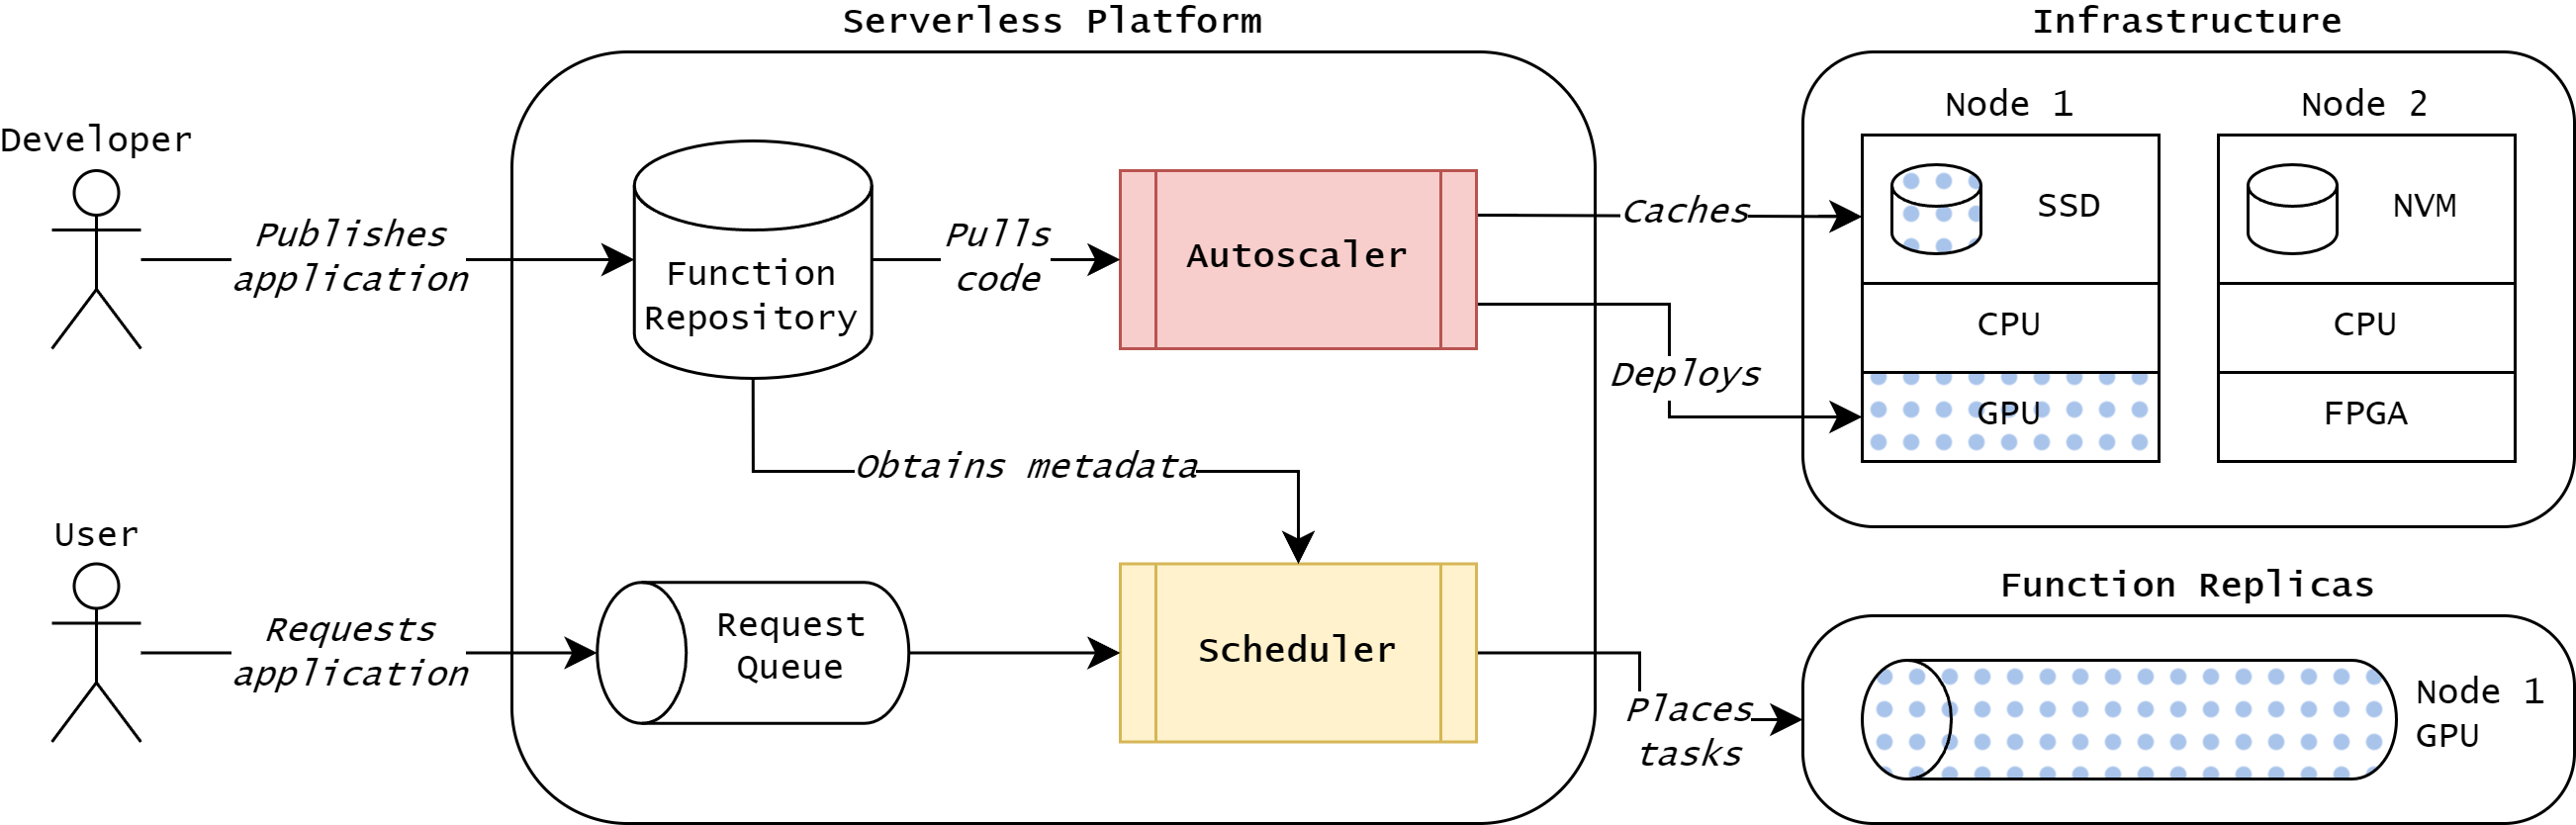
\includegraphics[width=0.9\textwidth]{7_Chapitre5/figures/platform.png}
    \caption{Vue de haut niveau d'une plateforme serverless, telle que modélisée dans HeROsim. L'autoscaler alloue des ressources matérielles pour les répliques de fonctions ; tandis que l'ordonnanceur place les requêtes utilisateur en file d'attente sur ces répliques}.
\label{figure:herosim-platform}
\end{figure*}

Dans le cloud, les clients réservent généralement des ressources. Il s'agit généralement d'un sous-ensemble virtualisé de ressources matérielles hétérogènes disponibles sur des serveurs appelés nœuds. Une fois la réservation effectuée, les fournisseurs de services offrent un accès à distance au client, qui est responsable du déploiement de ses applications et facturé en fonction de la quantité de ressources qu'il a réservées~\cite{Lannurien2023}.

Dans le paradigme serverless, les clients commencent par pousser leur code dans un référentiel du côté du fournisseur, voir la figure~\ref{figure:herosim-platform}. Le fournisseur alloue des ressources qui sont automatiquement mises à l'échelle en fonction de la charge. Pour que ce mécanisme fonctionne, les applications sont divisées en petites unités d'exécution sans état appelées \textbf{fonctions}. Ces fonctions sont sans état : si elles produisent des données de sortie, celles-ci doivent être conservées dans un stockage persistant~\cite{yuFollowingDataNot}.

Dans les modèles de service traditionnels, les ressources sont mises à l'échelle sur deux dimensions : horizontalement (nouvelles instances d'application créées sur d'autres nœuds) et verticalement (ressources supplémentaires allouées aux instances existantes). Dans les plateformes serverless, les ressources sont mises à l'échelle horizontalement : les variations de charge des applications sont absorbées par l'ajout de nouvelles instances des fonctions, appelées \textbf{replicas}, et leur suppression lorsqu'elles ne sont plus nécessaires. Une réplique peut être créée pour chaque requête utilisateur ou réutilisée pour plusieurs requêtes d'utilisateurs. Nous pouvons considérer les répliques de fonctions comme des files d'attente de requêtes ayant des capacités différentes.

Ces répliques sont créées par l'\textbf{autoscaler}. Pour gérer le nombre de répliques déployées pour chaque fonction, il existe trois stratégies principales : basée sur les requêtes, basée sur la concurrence et basée sur les métriques~\cite{mahmoudiSimFaaSPerformanceSimulator2021}. Dans le cadre de l'autoscaling basé sur les requêtes, les requêtes arrivant dans le système sont traitées par des répliques inactives. Si aucune réplique inactive n'est disponible, une nouvelle instance est créée. Dans l'autoscaling basé sur la concurrence, chaque réplique peut mettre en file d'attente plusieurs requêtes d'utilisateurs et les traiter séquentiellement en fonction d'un seuil de concurrence prédéfini~\cite{herofake}. Dans l'autoscaling basé sur les métriques, le nombre de répliques déployées dépend de divers objectifs, tels que le taux de requêtes par seconde (RPS) à atteindre. Pour ce faire, il faut surveiller les performances du système à l'usage de l'autoscaler.

Les répliques peuvent se trouver dans trois états différents : initialisation, exécution et inactivité~\cite{SchleierSmith2021WhatSC}. Lorsqu'une réplique de fonction vient d'être créée, elle est en état d'initialisation : la plateforme instancie son environnement d'exécution, extrait son code d'un registre distant et le met éventuellement en cache sur le nœud de déploiement, puis commence à exécuter la fonction. Lorsque la réplique traite les requêtes utilisateur, elle est en état d'exécution. Dans le cas contraire, la réplique est inactive et peut être supprimée. Lorsque les répliques sont supprimées, les ressources matérielles sont libérées. Toutefois, la création d'une nouvelle réplique pour traiter les requêtes utilisateur entraîne un surcoût appelé \textbf{démarrage à froid}. Les orchestrateurs adoptent diverses politiques pour atténuer ce problème, allant de l'application d'une période de maintien en vie sur les répliques de fonctions pour éviter de les détruire trop tôt, à l'allocation proactive de répliques.

Enfin, les requêtes utilisateur sont attribuées aux répliques de fonctions disponibles par l'\textbf{ordonnanceur} qui met en œuvre différentes stratégies : par exemple AWS Lambda\footnote{\href{https://aws.amazon.com/en/lambda/}{https://aws.amazon.com/en/lambda/}} utilise un algorithme de bin-packing, tandis qu'une plateforme open source telle que Knative met en œuvre une politique d'équilibrage de la charge~\cite{Lannurien2023}. Ces stratégies ont des résultats différents en ce qui concerne l'utilisation des ressources et la qualité de service, mais il peut être difficile de prédire dans quelle mesure elles auront un impact sur les charges de travail avant le déploiement.

\section{Choix de conception}
\label{section:herosim-herosim}

Cette section présente les choix de conception et les hypothèses formulées pour le développement de HeROsim.

\begin{figure}[t]
    \centering
    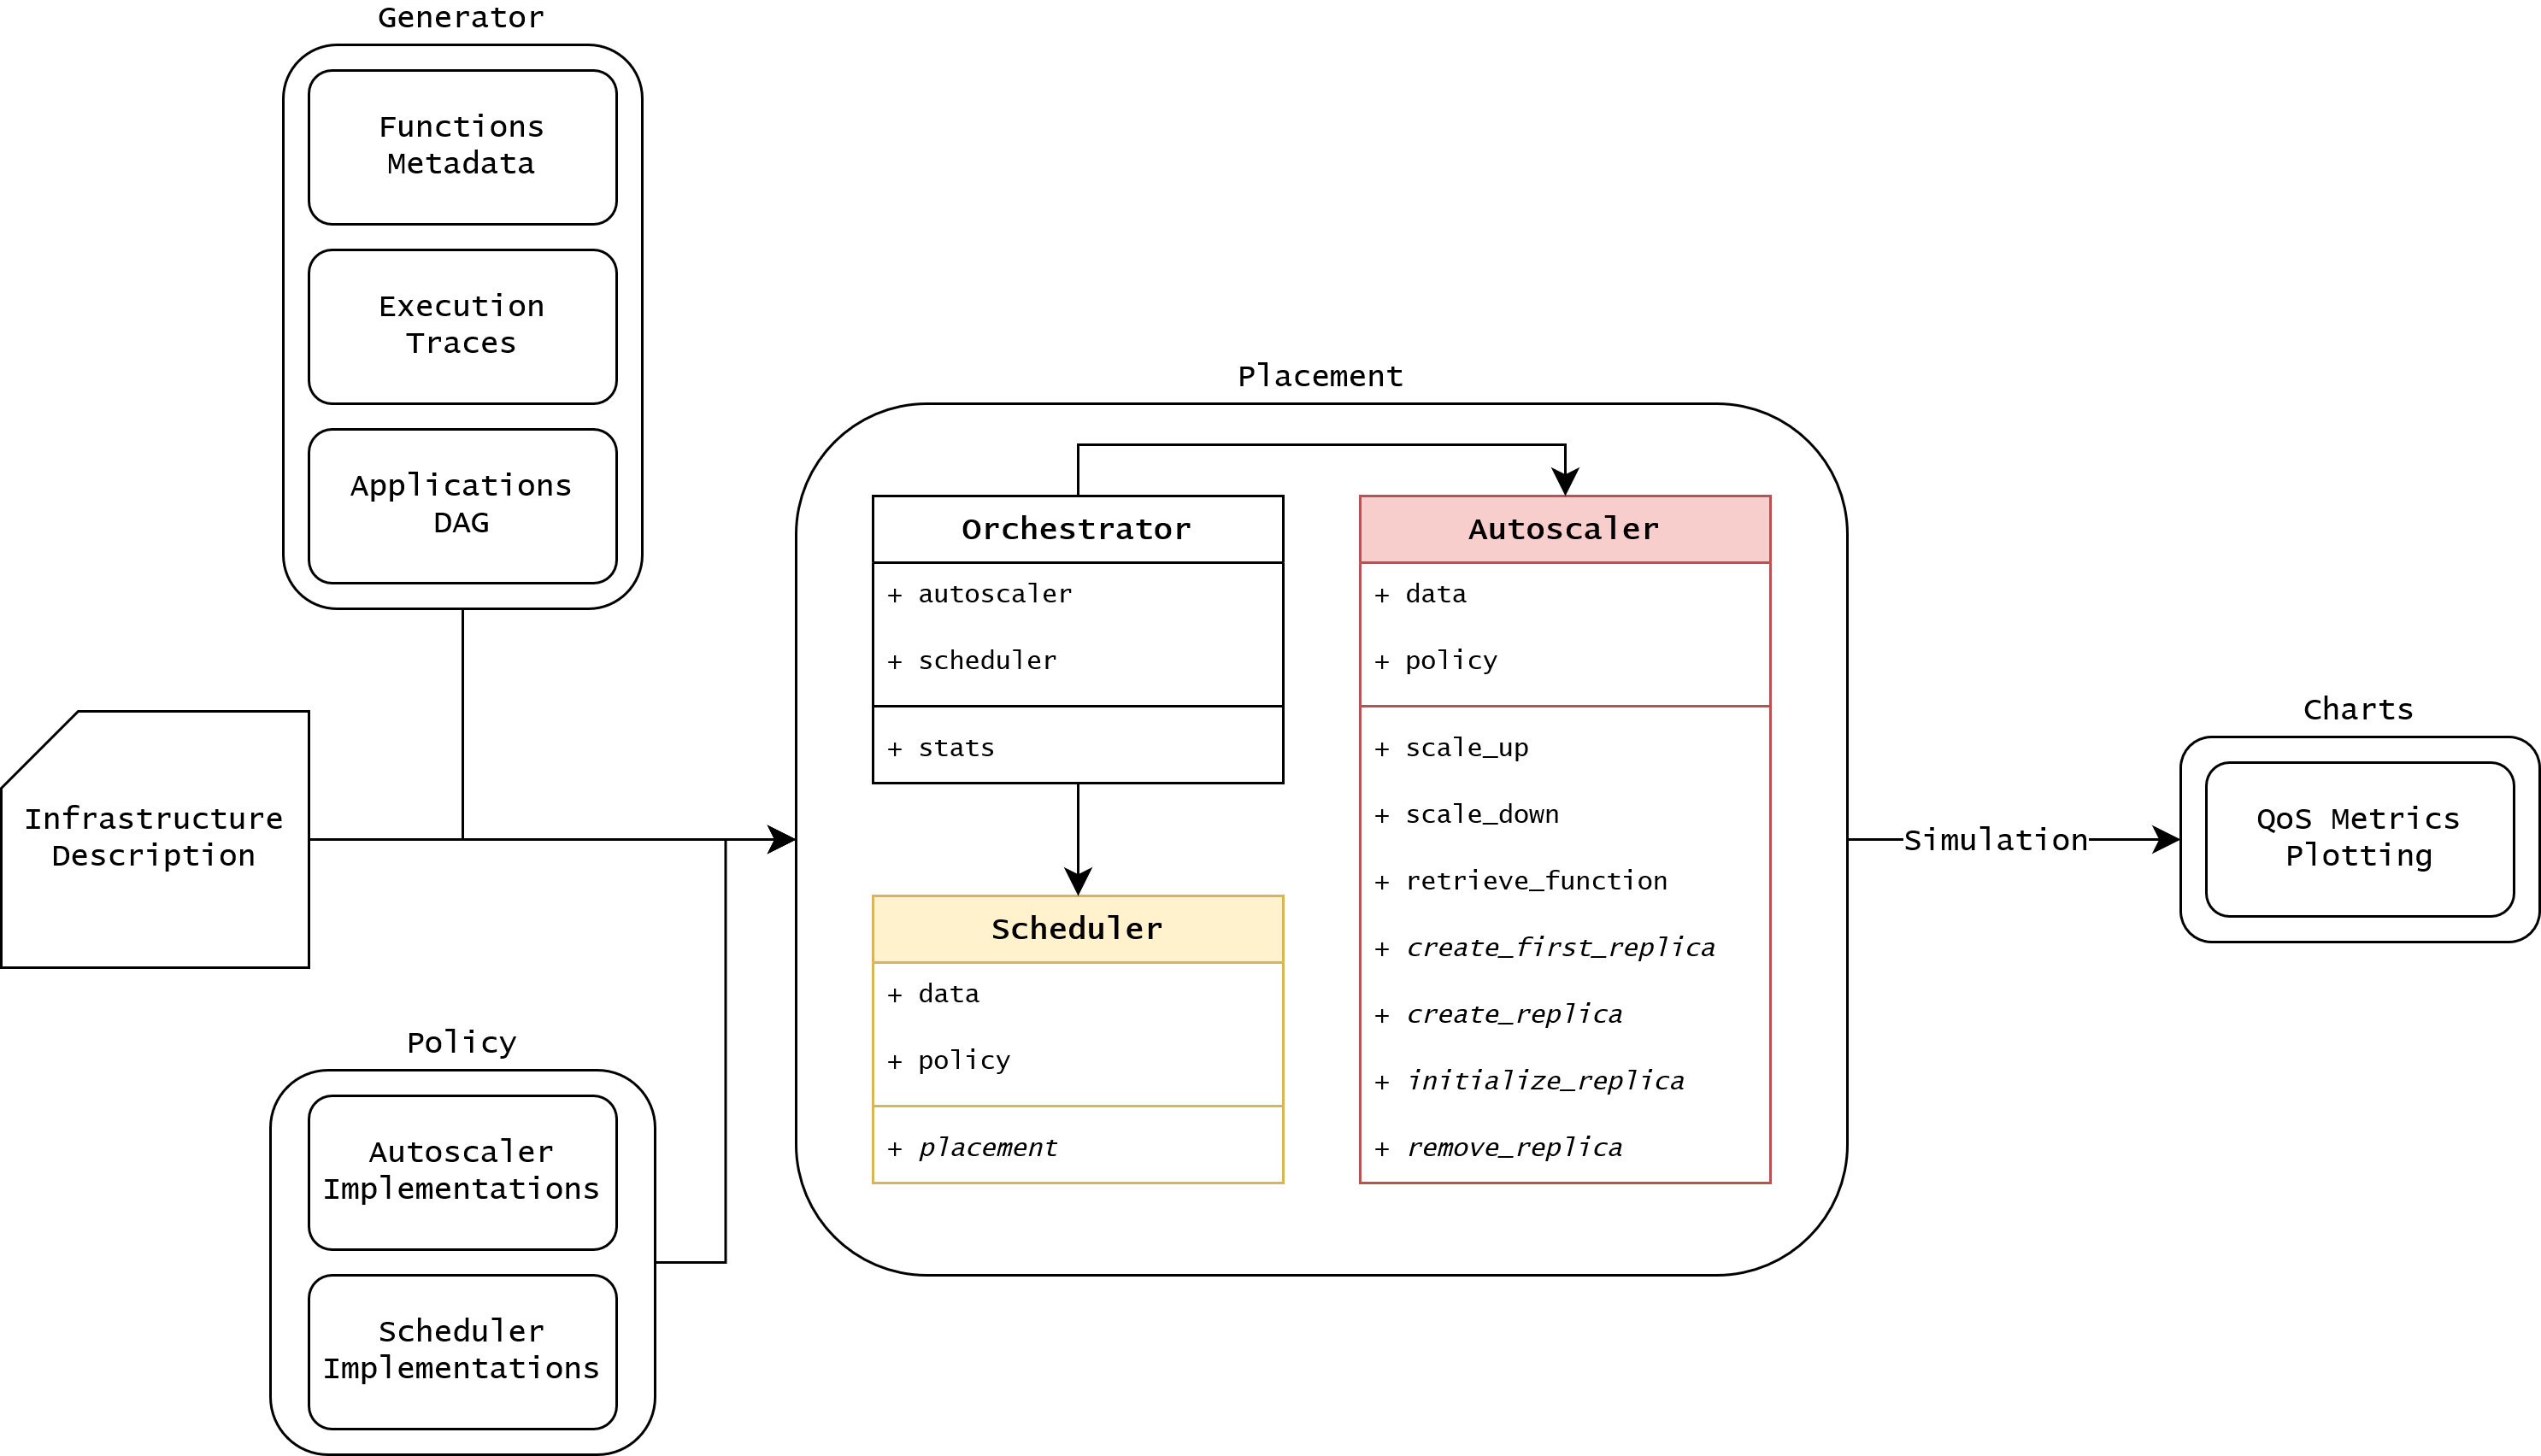
\includegraphics[width=\columnwidth]{7_Chapitre5/figures/software-architecture.png}
    \caption{Vue de haut niveau de l'architecture du simulateur.}
\label{figure:herosim-software-architecture}
\end{figure}

HeROsim utilise la bibliothèque SimPy~\footnote{\href{https://simpy.readthedocs.io}{https://simpy.readthedocs.io}} comme moteur de simulation à événements discrets. Il fournit trois classes de base - \texttt{Orchestrator}, \texttt{Autoscaler} et \texttt{Scheduler} - qui devraient être sous-classées par les utilisateurs désireux d'implémenter leurs propres algorithmes. Comme l'essentiel du comportement de la plateforme est hérité des classes de base, le coût de mise en œuvre d'une nouvelle politique est minime : le couple le plus simple d'autoscaler et d'ordonnanceur (politique de placement aléatoire) est mis en œuvre en moins de 20 lignes de code.

\subsection{Données d'entrée}

HeROsim expose une interface déclarative permettant aux utilisateurs de définir leur environnement cloud, leurs charges de travail et leurs contraintes de qualité de service. Le simulateur reproduit un scénario d'allocation et de placement selon différentes politiques d'orchestration. Une exécution du simulateur nécessite les entrées JSON suivantes pour définir un tel scénario :

\begin{enumerate}
    \item Une \textbf{description des applications} comportant les mesures des des \textbf{caractéristiques des fonctions} invoquées au cours du scénario, \textit{i.e.} leurs temps d'exécution et de démarrage à froid, leurs besoins mémoire, leur consommation d'énergie, la taille de l'image des fonctions, la taille des entrées/sorties lors des phases de communication. Ces métadonnées peuvent être définies en \textbf{mesurant} et \textbf{analysant} le comportement des applications sur une configuration de banc d'essai (voir figure~\ref{figure:herosim-characterization}) ;
    \item Une \textbf{description de l'infrastructure} listant les différents \textbf{nœuds disponibles} et les plateformes d'exécution qu'ils comportent, leurs supports de stockage et la bande passante disponible sur le réseau. Les plateformes d'exécution sont définies en termes de consommation d'énergie au repos et de prix de détail ; les dispositifs de stockage sont caractérisés par leur capacité, leur bande passante et leur latence. Ces données sont spécifiques à une plateforme cible et peuvent être \textbf{mesurées} ou obtenues auprès des fabricants ;
    \item Une \textbf{trace d'exécution} faisant état des temps d'arrivée pour toutes les \textbf{requêtes utilisateur} vers les applications déployées, associées au niveau de qualité de service demandé par l'utilisateur, dans l'ordre chronologique. Ces données peuvent être extraites par \textbf{observations} réelles des applications en production (voir figure~\ref{figure:herosim-characterization}), ou estimées statistiquement.
\end{enumerate}

Les données de nos études précédentes~\cite{herofake, herocache} sont disponibles dans le référentiel pour référence. Alors que (1) et (2) peuvent être rédigés à la main en fonction des exigences du cas d'utilisation, HeROsim fournit un générateur synthétique pour créer diverses traces pour (3) en utilisant des processus de Poisson, avec une durée variable et un taux requêtes par seconde, comme cela est couramment fait dans la littérature~\cite{herocache}. 

\subsection{Flot d'une simulation}

L'utilisateur peut choisir les politiques d'orchestration souhaitées et exécuter le programme principal. Le simulateur :

\begin{itemize}
    \item Initialise l'infrastructure comme décrit : le scénario commence avec tous les nœuds inactifs, en attente de nouvelles requêtes ;
    \item Initialise l'orchestrateur avec l'autoscaler et l'ordonnanceur choisis ;
    \item Suit les temps d'arrivée des événements à partir de la trace d'exécution et transmet les requêtes utilisateur à l'orchestrateur ;
    \item Laisse l'ordonnanceur essayer de placer ces requêtes sur des répliques de fonctions ;
    \item Laisse l'autoscaler allouer et désallouer les ressources matérielles qui hébergent ces répliques pour traiter les requêtes utilisateur.
\end{itemize}

La simulation progresse dans le traitement des requêtes utilisateur. Le simulateur connaît le temps de réponse des fonctions sur la base des métadonnées d'entrée mesurées au préalable. Ces métadonnées concernent le matériel et les charges de travail spécifiques que l'utilisateur souhaite ordonnancer. Elles peuvent être obtenues de différentes manières ; la figure~\ref{figure:herosim-characterization} donne un aperçu de la méthodologie que nous avons utilisée pour caractériser les différentes charges de travail et plates-formes d'exécution tout au long de nos expériences ; voir~\cite{herofake, herocache} pour plus de détails.

\begin{figure}[t]
    \centering
    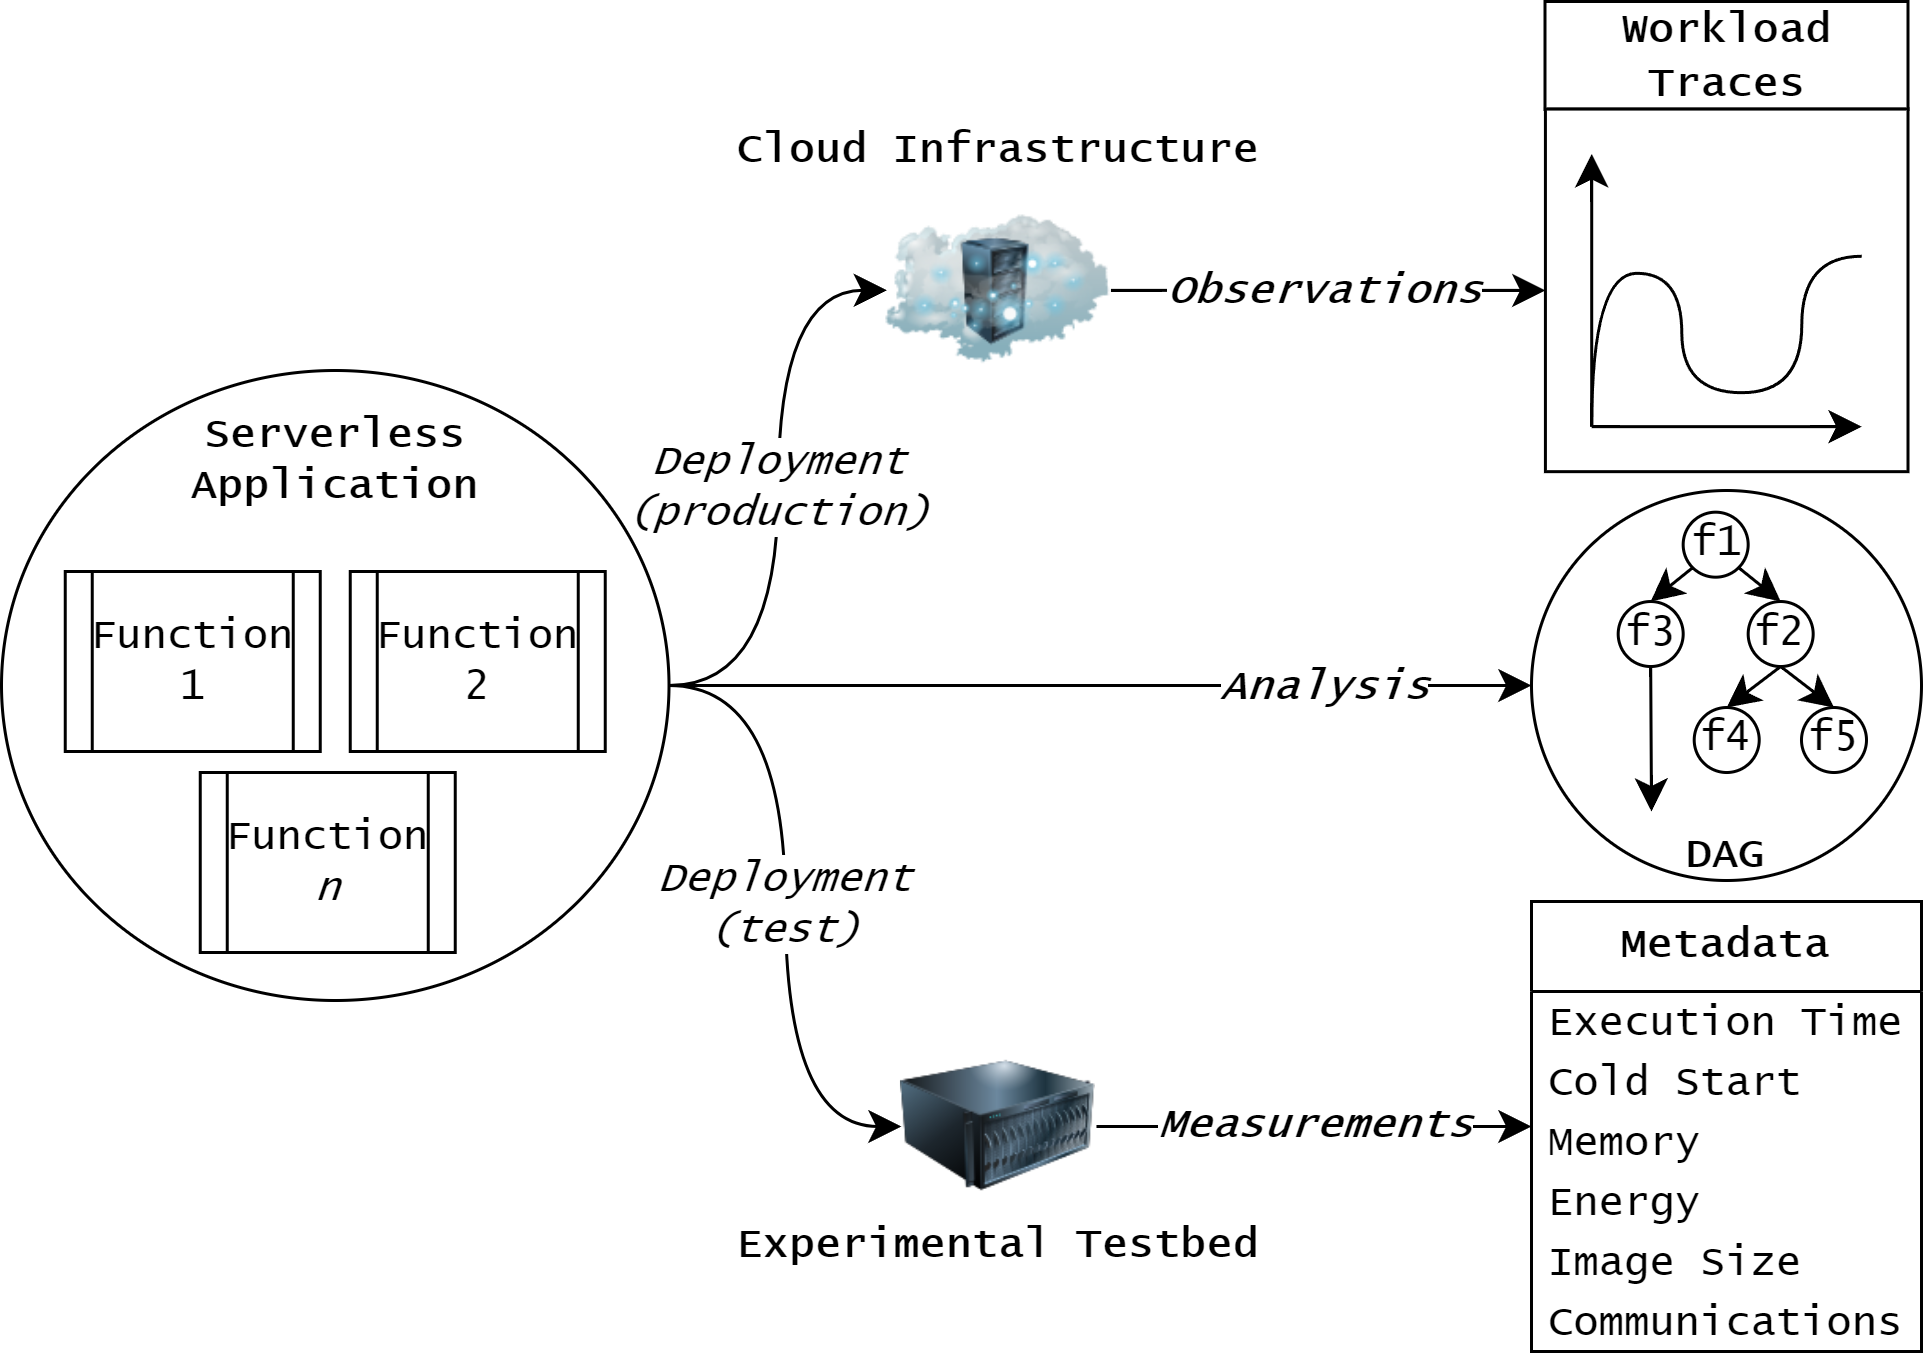
\includegraphics[width=\columnwidth]{7_Chapitre5/figures/characterization.png}
    \caption{Une vue d'ensemble de notre méthodologie de caractérisation.}
\label{figure:herosim-characterization}
\end{figure}

Pendant la simulation, les journaux sont écrits sur le disque. Lorsque toutes les requêtes utilisateur ont été traitées, la simulation s'arrête et renvoie les résultats et les graphiques résumant la simulation, respectivement dans les répertoires \texttt{result} et \texttt{chart}.

Le simulateur est monotâche, ce qui signifie que chaque politique sera évaluée de manière séquentielle. Cependant, plusieurs instances de HeROsim peuvent être exécutées en parallèle avec différentes configurations sur plusieurs cœurs de CPU, ou distribuées sur plusieurs nœuds. Chaque instance de HeROsim exécutant une politique d'orchestration différente et toutes les instances utilisant un répertoire de sortie commun, cela peut accélérer la durée totale du scénario de simulation lors de l'évaluation de nombreuses politiques d'orchestration. Lorsque toutes les exécutions du simulateur sont terminées, les résultats peuvent être consolidés dans un seul tableau de sortie.

\subsection{Orchestrateur}

La classe de base \textbf{\texttt{Orchestrator}} fournit des méthodes d'initialisation abstraites qui doivent être surchargées pour gérer différentes structures de l'état du système. Par exemple, un ordonnanceur Round Robin devra savoir combien de fois chaque réplique de fonction a été sélectionnée pour le placement des tâches, tandis qu'un ordonnanceur Least Connected devra connaître la concurrence moyenne dans chaque réplique pour équilibrer la charge. Cette classe est le point d'entrée permettant aux utilisateurs de définir leurs propres structures de données qui représenteront au mieux l'état du système à gérer par l'autoscaler et l'ordonnanceur.

Les utilisateurs peuvent mettre en œuvre le processus de gestion de l'état du système dont ils ont besoin pour soutenir leurs politiques d'orchestration. L'orchestrateur de base est doté d'un système simple qui peut fonctionner tel quel ou être étendu. Dans notre implémentation, un processus de surveillance est appelé périodiquement pour garder une trace de la concurrence moyenne dans chaque réplique de fonction. Ceci est utile pour les politiques basées sur des seuils.

La méthode du point d'entrée de l'orchestrateur est appelée chaque fois qu'une requête utilisateur arrive sur la plateforme. Elle prend en entrée l'état du système et la requête utilisateur. Elle peut être surchargée dans chaque implémentation de politique d'orchestration pour permettre une mise à l'échelle automatique et une ordonnanceur à grain fin selon les besoins.

Enfin, cette classe est responsable de l'instanciation des implémentations sélectionnées pour \texttt{Autoscaler} et \texttt{Scheduler}. Toute combinaison de ces deux modules peut être instanciée.

\subsection{Allocateur}

La classe de base \textbf{\texttt{Autoscaler}} fournit le comportement commun de la plateforme d'autoscaling, y compris la création et la suppression des répliques de fonctions. Plusieurs méthodes abstraites doivent être remplacées pour mettre en œuvre une nouvelle politique : sélection des ressources pour la création de répliques, processus d'initialisation des répliques, sélection des répliques pour la suppression, etc. Ces méthodes opèrent à la granularité d'une seule fonction, en prenant l'état du système et la liste des ressources matérielles disponibles comme données d'entrée. Les utilisateurs sont libres de mettre en œuvre les algorithmes qu'ils souhaitent évaluer pour la gestion des ressources.

L'autoscaler de HeROsim a été principalement conçu pour une mise à l'échelle horizontale. Les répliques de fonctions sont créées en allouant une plateforme d'exécution et la quantité requise de mémoire de crête sur un nœud. Une plateforme d'exécution ne peut pas héberger plus d'une réplique de fonction à la fois. Pour faire face à l'augmentation de la charge d'une application sans dégradation de la qualité de service, de nouvelles répliques de fonctions doivent être allouées par l'autoscaler, à condition qu'il y ait suffisamment de ressources matérielles disponibles. Les répliques nouvellement allouées passent par une phase d'initialisation au cours de laquelle les images des fonctions doivent être récupérées via le réseau. L'autoscaler peut gérer un cache d'images dans la mémoire du nœud et sur le stockage local du nœud afin d'accélérer les démarrages à froid.

La suppression des répliques inactives se fait au mieux : l'autoscaler tente de supprimer les répliques dont les files d'attente de tâches sont vides. Par défaut, une réplique avec des tâches en attente ne peut pas être supprimée.

L'autoscaler garde une trace de chaque événement d'allocation pour calculer l'utilisation des ressources à la fin de la simulation. HeROsim permet à l'utilisateur de savoir quels nœuds et quelles plates-formes d'exécution ont été enrôlés pendant le scénario, à quel moment et pour quelle durée, et pour quel déploiement de fonction ils ont été choisis. Cela permet également à HeROsim de calculer la consommation d'énergie à différentes granularités : la puissance statique nécessaire au matériel alloué et la puissance dynamique utilisée par les applications pendant leur exécution.

HeROsim est livré avec les politiques de mise à l'échelle automatique suivantes, basées sur des seuils de concurrence et prêtes à l'emploi :

\begin{itemize}
    \item Random -- Sélectionne un nœud aléatoire et une plateforme d'exécution pour les nouvelles répliques ;
    \item Knative -- Sélectionne le nœud le moins chargé pour allouer de nouvelles répliques, \textit{i.e} équilibre les charges de travail sur un grand nombre de nœuds ;
    \item HeROfake -- Exploite l'hétérogénéité du matériel pour minimiser les pénalités de qualité de service, la consommation d'énergie et le coût total de possession. Plus de détails sont donnés dans la section "Étude de cas" ;
    \item HeROcache -- Optimise les allocations pour les chaînes de fonctions ; maximise les fonctions de consolidation de chaque application. Plus de détails sont donnés dans la section "Étude de cas".
\end{itemize}

\subsection{Ordonnanceur}

La classe de base \textbf{\texttt{Scheduler}} met en œuvre la sélection des tâches dans la file d'attente de la passerelle. Une méthode abstraite doit être surchargée pour mettre en œuvre une nouvelle politique : la sélection d'une réplique parmi le pool pour placer chaque requête utilisateur dans la file d'attente. Cette méthode opère à la granularité d'une requête utilisateur et prend en entrée l'état du système et la liste des répliques de fonctions disponibles.

Les requêtes utilisateur arrivent dans une file d'attente au niveau de l'ordonnanceur. Les utilisateurs peuvent mettre en œuvre leur propre politique de priorité pour la sélection des tâches ou choisir une politique déjà disponible dans le simulateur, \textit{e.} FIFO ou Earliest Deadline First~\cite{herofake}.

L'ordonnanceur de HeROsim a été conçu sans tenir compte des défaillances ou des migrations de tâches : le comportement par défaut considère les tâches qui s'exécutent toujours jusqu'à leur terme sur leur réplique. Cependant, les tâches seront marquées comme "en pénalité" si l'ordonnanceur manque son échéance. Les utilisateurs peuvent utiliser cette valeur booléenne pour évaluer la qualité de leurs politiques en ce qui concerne la latence des requêtes : elle indique la proportion de requêtes qui sont traitées en temps voulu. 

S'il n'y a pas de réplique disponible au moment de l'ordonnancement d'une requête utilisateur, l'ordonnanceur fera un appel à l'autoscaler pour forcer la création d'une première réplique pour la fonction. Dans l'intervalle, la requête est remise dans la file d'attente et reportée. Les tâches reportées sont signalées comme telles, de sorte que, par exemple, elles peuvent avoir une priorité plus élevée si l'utilisateur souhaite appliquer une telle politique~\cite{herocache}.

HeROsim est livré avec les politiques d'ordonnanceur suivantes implémentées et prêtes à l'emploi :

\begin{itemize}
    \item Random -- Sélectionne une réplique aléatoire pour le placement des tâches ;
    \item Knative -- Sélectionne la réplique avec la file d'attente la plus courte pour le placement des tâches ;
    \item BPFF -- Sélectionne la réplique avec la plus longue file d'attente de requêtes en vol pour le placement des tâches ;
    \item HeROfake -- Sélectionne la réplique qui minimise un score composé en fonction de l'échéance de la tâche, de la consommation d'énergie de la fonction et de la dispersion des tâches sur les nœuds. Plus de détails sont donnés dans la section "Étude de cas" ;
    \item HeROcache -- Sélectionne la réplique similaire à HeROfake, mais prend en compte les opérations de stockage et de communication pour calculer la latence de bout en bout de la requête, et prend en compte les chaînes de fonctions lors de l'évaluation des répliques en ce qui concerne la consolidation des tâches. De plus amples détails sont donnés dans la section "Étude de cas".
\end{itemize}


\subsection{Interface utilisateur}

HeROsim s'appuie sur la journalisation pour fournir un aperçu du déroulement de la simulation, ce qui aide l'utilisateur à déboguer ses politiques. À la fin de la simulation, les fichiers de résultats sont enregistrés sur le disque. Ces fichiers contiennent des informations sommaires sur les résultats de la simulation, y compris les performances de la politique en ce qui concerne les mesures d'évaluation. Ces résultats sont représentés sur différents graphiques qui peuvent être utilisés dans des publications ultérieures (voir figure~\ref{figure:herosim-evaluation}).

HeROsim peut également générer des graphiques supplémentaires qui peuvent être utiles lors du débogage du comportement d'une politique d'orchestration. Les utilisateurs peuvent visualiser la proportion de démarrages à froid et d'accès au cache parmi les invocations de fonctions. HeROsim peut tracer la latence de la queue pour toutes les requêtes des utilisateurs, aidant ainsi l'utilisateur à dimensionner son infrastructure. Le générateur de traces d'exécution trace les temps d'arrivée des requêtes sur un graphique afin de fournir des indications visuelles sur les caractéristiques de la charge de travail.

\begin{figure}[t]
    \centering
    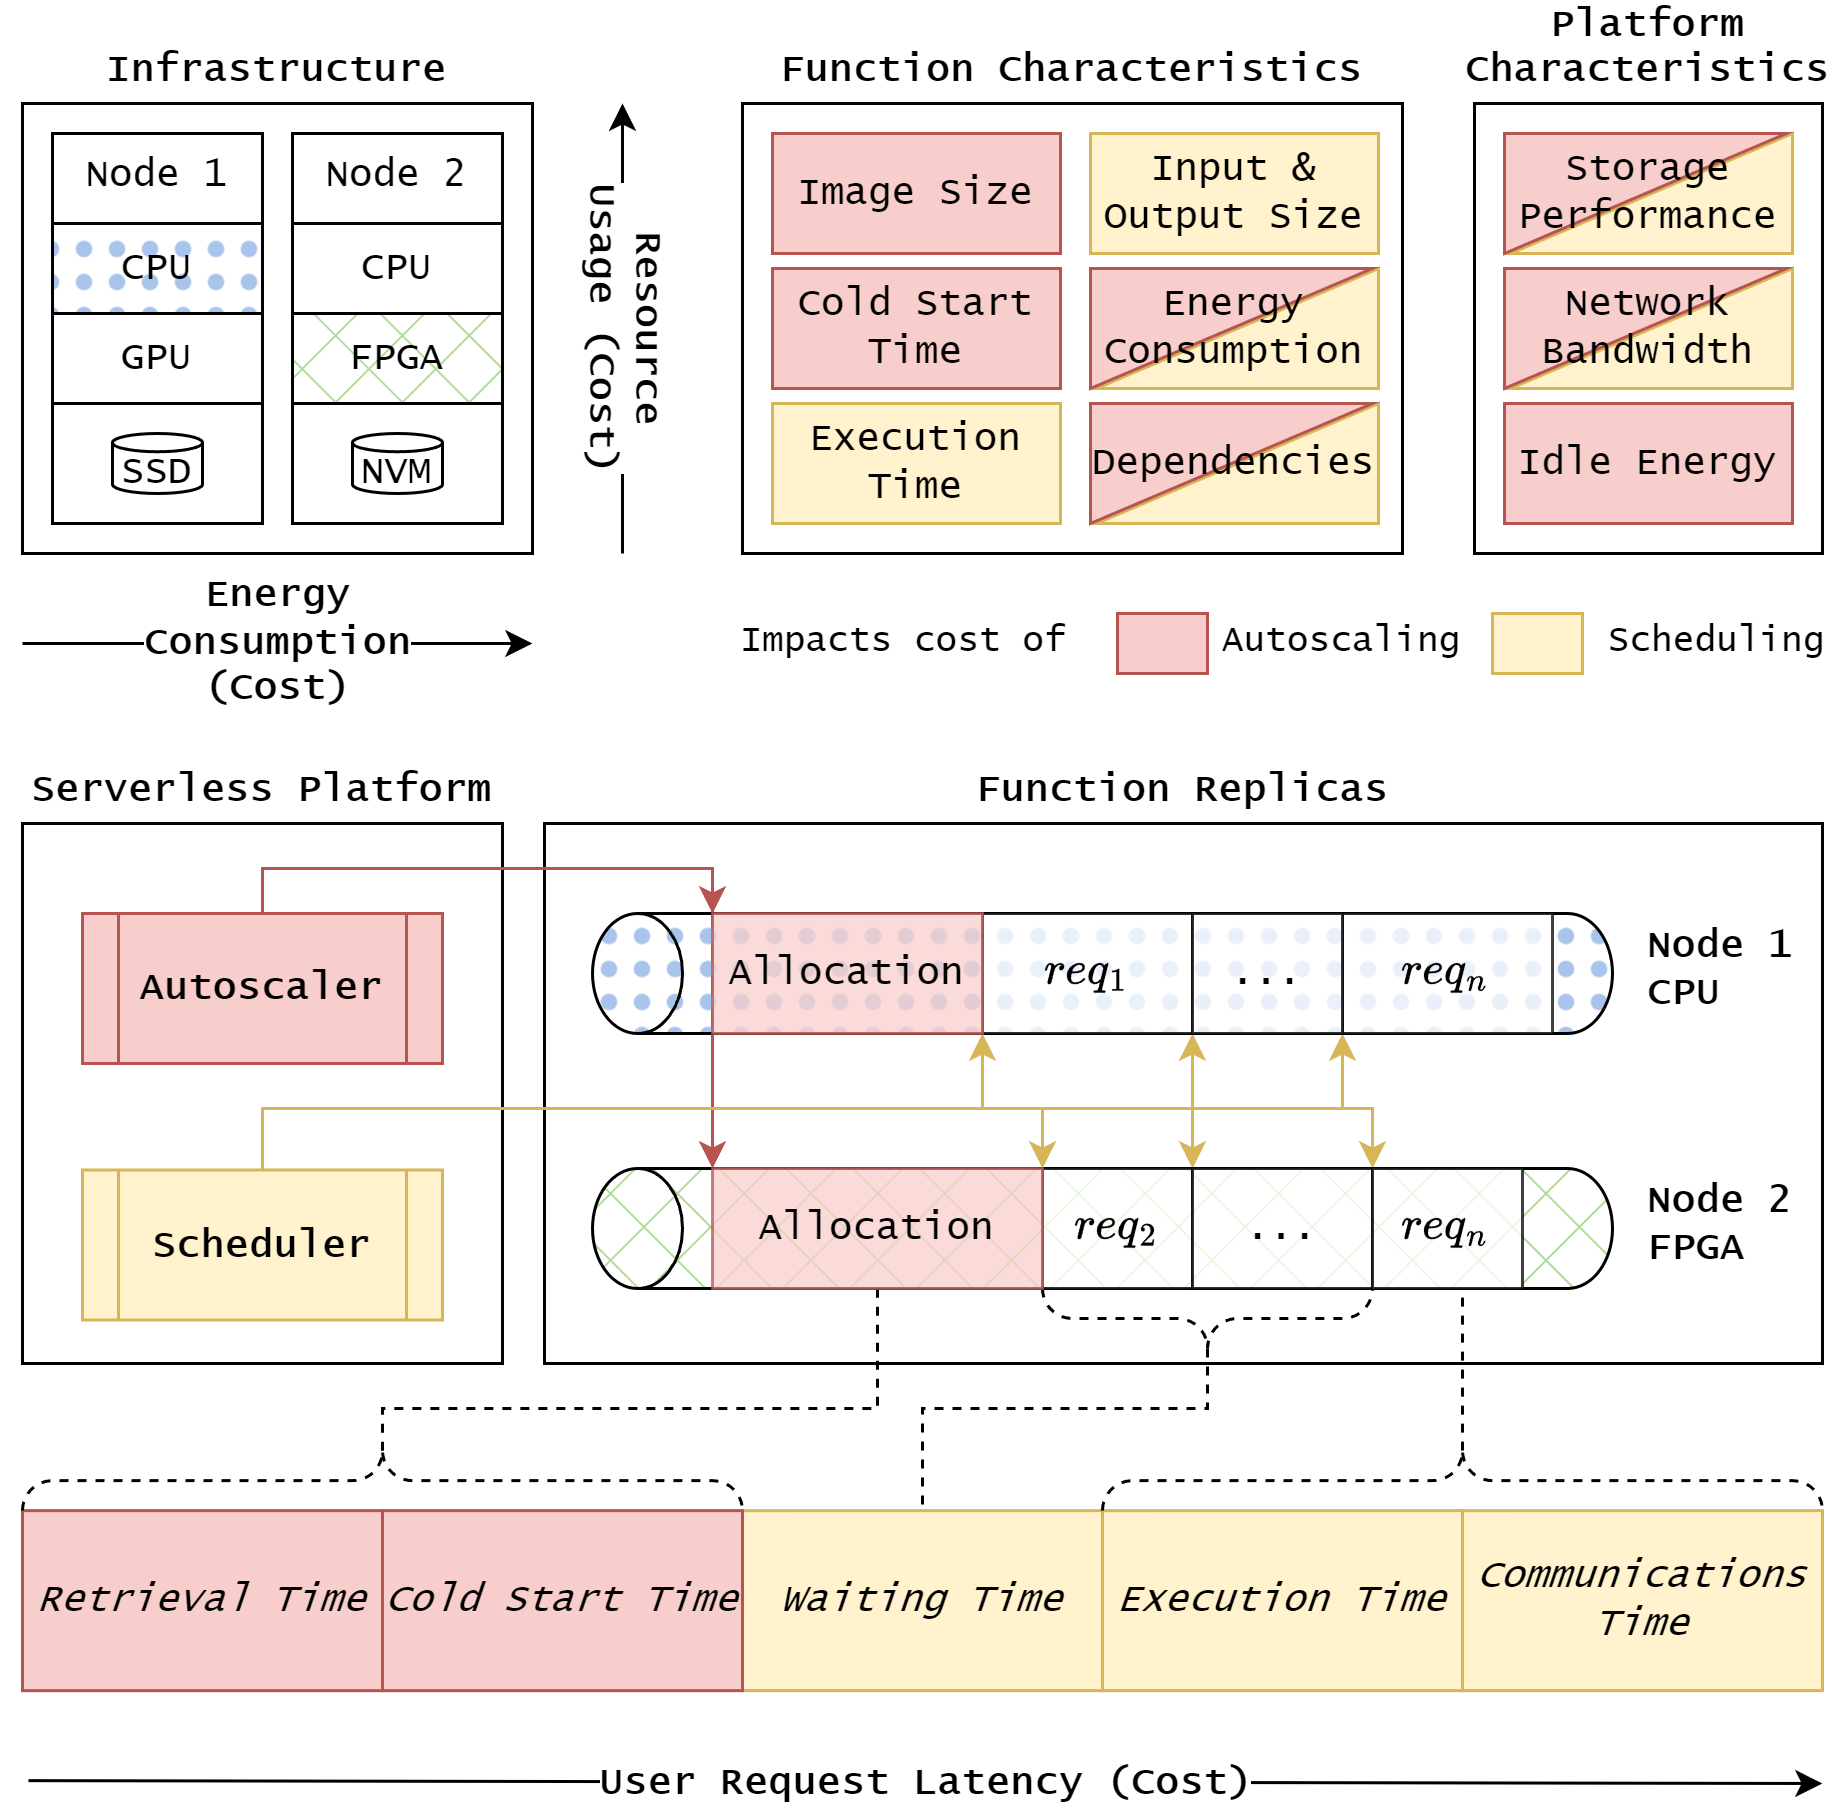
\includegraphics[width=\columnwidth]{7_Chapitre5/figures/serverless-cost.png}
    \caption{Répartition du coût de latence de bout en bout induit par les décisions d'autoscaling et d'ordonnancement.}
\label{figure:herosim-cost}
\end{figure}

\section{Étude de cas}
\label{section:herosim-case-study}

\begin{figure*}[t]
    \center
    \subfloat[Consolidation\label{figure:herosim-evaluation-full-unused-nodes}]{
        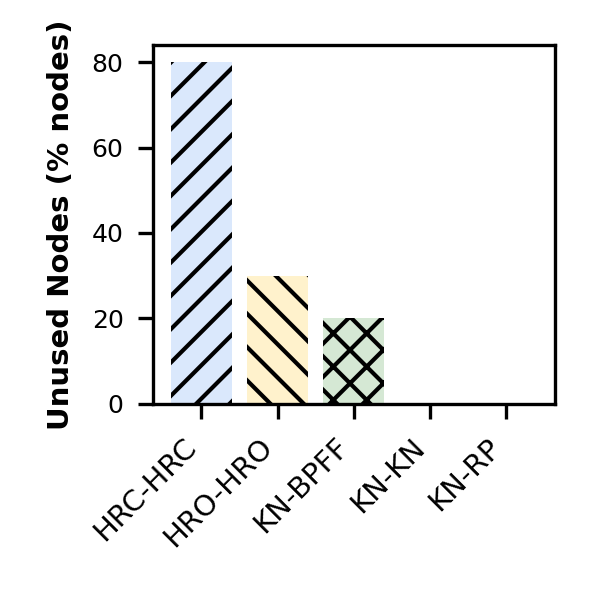
\includegraphics[width=0.155\linewidth]{7_Chapitre5/figures/eval/2-unused-nodes.png}
    }
    \subfloat[QoS\label{figure:herosim-evaluation-full-penalty}]{
        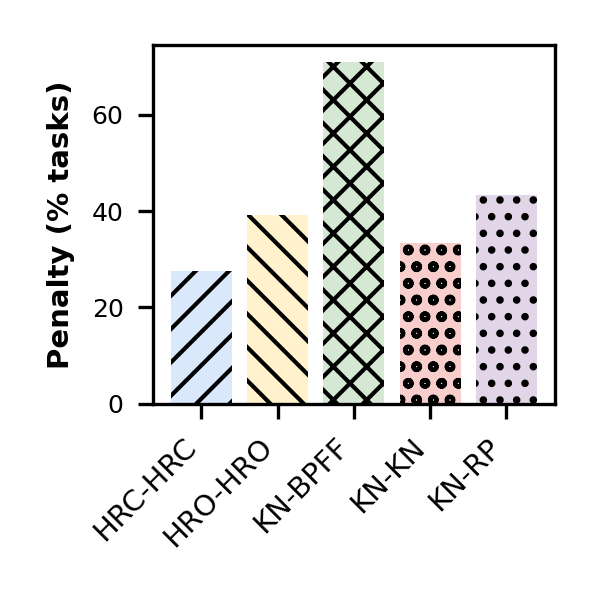
\includegraphics[width=0.155\linewidth]{7_Chapitre5/figures/eval/3-penalty-proportions.png}
    }
    \subfloat[Energy\label{figure:herosim-evaluation-full-energy-consumption}]{
        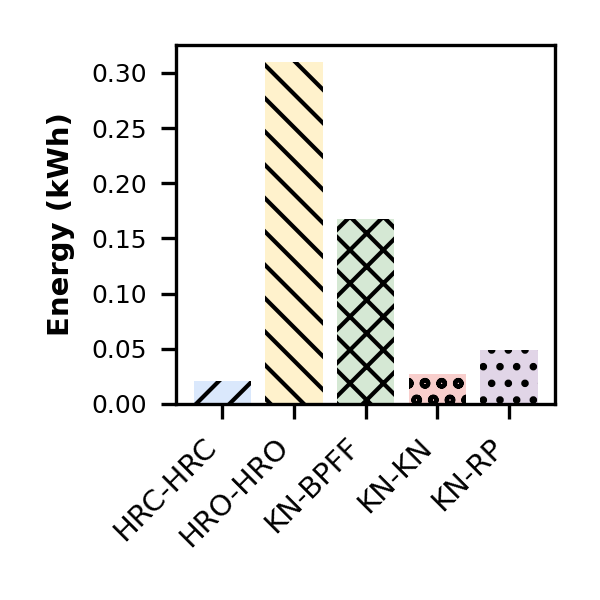
\includegraphics[width=0.155\linewidth]{7_Chapitre5/figures/eval/6-energy-consumption.png}
    }
    \subfloat[Consolidation\label{figure:herosim-evaluation-components-unused-nodes}]{
        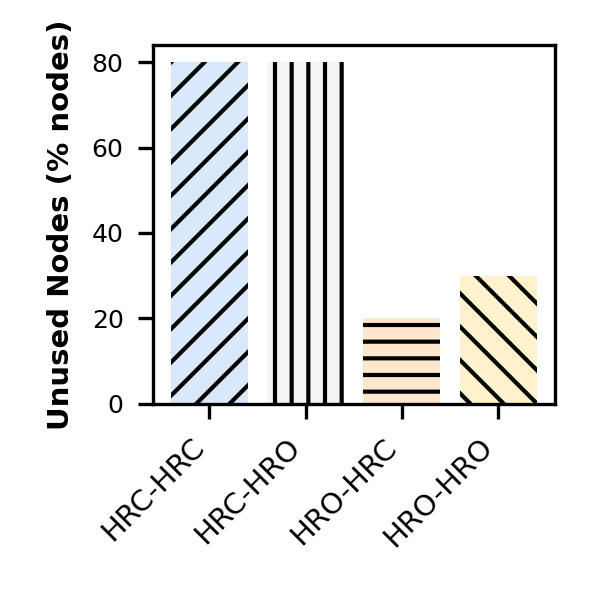
\includegraphics[width=0.155\linewidth]{7_Chapitre5/figures/eval-components/2-unused-nodes.png}
    }
    \subfloat[QoS\label{figure:herosim-evaluation-components-penalty}]{
        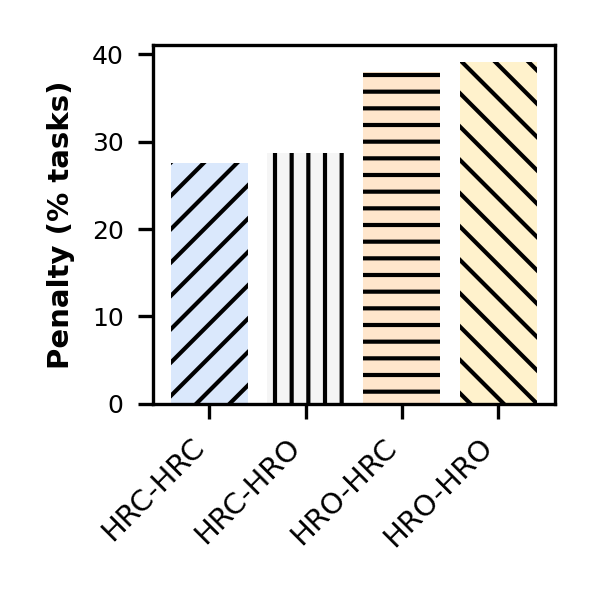
\includegraphics[width=0.155\linewidth]{7_Chapitre5/figures/eval-components/3-penalty-proportions.png}
    }
    \subfloat[Energy\label{figure:herosim-evaluation-components-energy-consumption}]{
        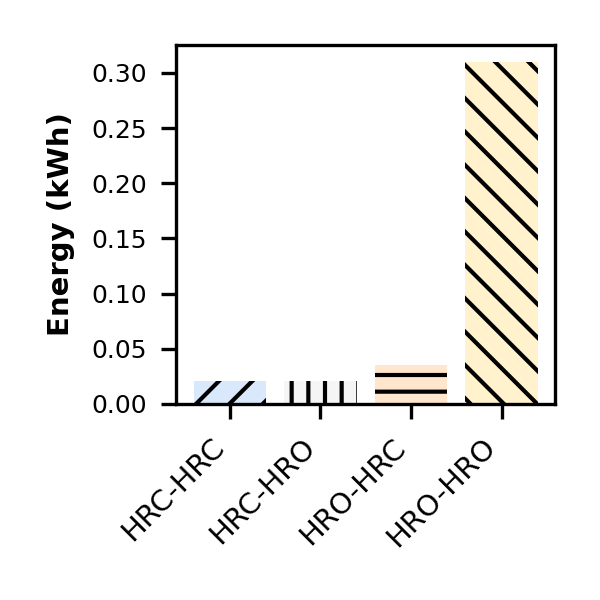
\includegraphics[width=0.155\linewidth]{7_Chapitre5/figures/eval-components/6-energy-consumption.png}
    }
    \caption{Charts generated by HeROsim for the evaluation of HeROcache -- Comparison against baselines (a-c) and impact of individual components (d-f). HRC-HRO means HeROcache autoscaler coupled with HeROfake scheduler.}
    \label{figure:herosim-evaluation}
\end{figure*}

Nous présentons deux études de cas qui ont utilisé HeROsim pour évaluer les politiques d'orchestration.
Nous avons conçu des stratégies qui reposent sur la caractérisation des plateformes hétérogènes et des charges de travail (voir figure~\ref{figure:herosim-characterization}). Nous avons mesuré plusieurs métriques liées à nos applications sur diverses plateformes matérielles et proposé un modèle de coût qui intègre ces valeurs pour estimer les performances de l'autoscaling et de l'ordonnanceur sous différentes politiques (figure~\ref{figure:herosim-cost}).

\subsection{Stratégie d'orchestration de fonctions sans état sur ressources hétérogènes}

Dans cette première étude de cas, \textbf{He}terogeneous \textbf{R}esources \textbf{O}rchestration for deep\textbf{fake} detection~\cite{herofake}, nous avons étudié le déploiement d'une application de détection de deepfake sur une plateforme serverless dans un cloud privé. En particulier, nous nous sommes intéressés à l'exploitation de ressources hétérogènes pour l'orchestration serverless lors de l'optimisation de la plateforme pour la QoS et la consommation d'énergie.

L'application exécute des tâches d'inférence pour détecter les deepfakes dans des images potentiellement trafiquées, soumises par des utilisateurs avec diverses exigences de niveau de QoS. Son objectif est de détecter les images potentiellement falsifiées, c'est-à-dire les images susceptibles d'avoir été manipulées par ordinateur pour tromper les spectateurs. Il se compose de trois tâches de réseau neuronal indépendantes et sans état qui ont été mises en œuvre sur du matériel hétérogène : CPU, GPU et FPGA. Ces implémentations ont été utilisées pour les mesures, mais il aurait été difficile d'exécuter réellement des scénarios du monde réel sur une plateforme serverless incluant ces architectures matérielles.

Dans HeROfake, chaque exécution de tâche a un coût associé mesuré en \textbf{latence}. L'allocation de nouvelles répliques sur des ressources matérielles inactives introduit un \textbf{délai de démarrage à froid} ; le traitement des requêtes utilisateur sur différents matériels a divers \textbf{temps d'exécution de la fonction}. La latence de chaque requête utilisateur est finalement comparée à la \textbf{exigence de qualité de service} de la requête : si l'échéance de la requête n'a pas été respectée, la tâche est en \textbf{pénalité}. Ces éléments constituent la base de notre modèle de coût, voir la figure~\ref{figure:herosim-cost}.

Les différentes architectures matérielles ont également des coûts monétaires et énergétiques différents qui ont été pris en compte dans le modèle de coût. Nous avons mis en œuvre un autoscaler et un ordonnanceur qui cherchent à estimer et à minimiser ce coût composite à la granularité de chaque requête utilisateur. L'autoscaler cherche à allouer des plateformes qui minimisent le coût global, y compris l'utilisation des ressources, la consommation d'énergie et le coût total de possession. L'ordonnanceur cherche à sélectionner les répliques qui traitent les requêtes avec le moins de pénalités et la plus faible consommation d'énergie.

HeROfake a été évalué à l'aide d'un scénario synthétique avec une distribution uniforme des temps d'arrivée des requêtes, des appels de fonction et des niveaux de qualité de service. HeROfake s'est avéré performant (en termes de pénalités de QoS, de consolidation et d'énergie) par rapport à Knative (l'orchestrateur serverless de Google) et Bin-Packing First Fit (la politique d'Amazon dans Lambda)~cite{herofake}. 

Notre objectif principal était d'étudier la pertinence de la prise en compte de l'hétérogénéité matérielle lors de l'allocation des ressources et de l'ordonnancement des requêtes utilisateur en ce qui concerne diverses mesures de qualité de service, \textit{i.e.} la latence de bout en bout et la consommation d'énergie. Les résultats expérimentaux ont montré que si le temps total d'exécution des tâches dans HeROfake est similaire à celui de la version vanille de Knative, nous obtenons une réduction de plus de 60\% des pénalités de qualité de service ; les tâches sont consolidées sur moins de 40\% des nœuds de l'infrastructure, 77\% des plates-formes d'exécution restant inutilisées ; et la consommation d'énergie dynamique est réduite de 35\% par rapport à Knative.

HeROsim nous a également permis d'évaluer l'impact des différents composants de notre cadre. Les résultats ont montré que, même en allouant uniquement des CPU, l'ordonnanceur des tâches d'inférence avec notre politique consciente de la qualité de service pouvait maintenir les violations des accords de niveau de service en dessous de 50\%. 

\subsection{Stratégie d'orchestration d'applications avec prise en compte du cache et des communications}

Ici, une stratégie d'orchestration consciente des contraintes temporelles et de données a été proposée. Nous avons exploré le déploiement d'un système de détection d'intrusion (IDS) sur une plateforme serverless. En particulier, nous avons étudié les avantages de l'orchestration consciente des données lors de l'exploitation de matériel hétérogène pour déployer des applications sensibles au temps sur des dispositifs périphériques à ressources limitées, du point de vue du fournisseur de services.

L'objectif de l'application est de détecter le trafic TCP potentiellement malveillant dans les journaux de réseau soumis par les utilisateurs. Comme cette application IDS est spécifiquement destinée aux missions de drones, son schéma d'accès est étroitement lié aux schémas saisonniers, ce qui en fait une bonne adaptation au paradigme serverless.

L'application se compose de deux couches : deux fonctions de prétraitement qui opèrent sur les journaux du trafic réseau, et quatre fonctions d'inférence qui détectent des modèles d'activité malveillante dans les journaux. Ces fonctions ont été mises en œuvre sur différentes architectures matérielles (CPU, FPGA, GPU). 

Il existe des dépendances de données entre les deux couches de l'application. Nous les avons modélisées sous forme de graphes acycliques dirigés (DAG) d'appels de fonctions. Nous avons utilisé le module Python \texttt{TopologicalSorter} du module \texttt{graphlib} pour la représentation JSON des graphes et pour les parcourir pendant l'exécution.

Au niveau de l'orchestrateur, nous avons dû modifier la granularité des requêtes utilisateur : une requête concerne une application, qui peut être composée d'une ou plusieurs fonctions, appelées dans l'ordre défini par le DAG de l'application. Chaque fonction peut prendre des données en entrée et produire des données en sortie. Ces données sont définies par leur taille en octets.

Alors que HeROfake ne prend pas en compte les opérations de stockage, HeROcache met en œuvre la \textbf{récupération des images de fonctions}, \textbf{la mise en cache des images de fonctions} et les \textbf{communications entre fonctions} dans l'orchestrateur de base. Ces opérations augmentent la latence de la requête utilisateur d'une quantité de temps calculée sur la base de la caractérisation de la plateforme et de la fonction, voir figure~\ref{figure:herosim-cost} : par exemple, HeROsim estime le temps de récupération de l'image de la fonction sur la base de la largeur de bande du réseau spécifiée par l'utilisateur dans la description de l'infrastructure, la taille de l'image de la fonction spécifiée par le type de charge de travail, et la performance du stockage local du nœud spécifiée par le type de stockage.

L'introduction d'opérations de stockage au niveau du nœud individuel nous a permis d'évaluer une stratégie de préchargement d'images de fonctions afin d'accélérer les démarrages à froid dans les invocations futures.

Dans HeROcache, l'autoscaler cherche à accroître la consolidation des fonctions entre les applications, à réduire le makespan global, la consommation d'énergie et le coût total de possession. L'ordonnanceur cherche à éviter le non-respect des délais des requêtes, à consommer moins d'énergie et à assurer une utilisation élevée des ressources.

Nous avons utilisé le générateur de traces d'exécution inclus dans HeROsim pour générer un scénario de 30 minutes de requêtes utilisateur suivant un processus de Poisson à un taux moyen de 83 requêtes par seconde. Cela correspond au taux de communication que la connectivité 4G LTE permettrait dans notre environnement périphérique, compte tenu de la taille des données d'entrée et de sortie de l'application. 

HeROfake exploite déjà l'hétérogénéité matérielle, mais est conçu comme une politique sans stockage, ce qui en fait une solution comparable. Cette comparaison nous a permis de montrer l'importance des coûts de stockage dans le respect de la qualité de service : avec une politique d'orchestration tenant compte des données, HeROcache consolide les applications et parvient à réduire les délais d'initialisation moyens de 17,6 % et les délais de communication de 88,4 %. Cela permet de réduire la consommation d'énergie statique de la plateforme de 80 % tout en maintenant moins de 28 % de violations de la qualité de service.

HeROcache (mis en œuvre au-dessus de HeROsim) a été soumis à l'évaluation des artefacts et a reçu les trois badges de reproductibilité de l'IEEE~\footnote{\href{https://www.niso.org/standards-committees/reproducibility-badging}{https://www.niso.org/standards-committees/reproducibility-badging}} : Open Research Objects (ORO), Reusable/Research Objects Reviewed (ROR), et Results Reproduced (ROR-R).

\section{Travaux connexes}
\label{section:herosim-sota}

\begin{table*}[t]
    \centering
    \caption{Overview of simulation tools for cloud computing}
    \resizebox{\linewidth}{!}{
        \begin{tabular}{lSSSSSSSSS}
        \toprule
        & Serverless & Deployment models & Functions chains & Hardware heterogeneity & Per-request QoS & Resource usage & Energy consumption & Visualization \\
        \cmidrule(lr){2-2}\cmidrule(lr){3-3}\cmidrule(lr){4-4}\cmidrule(lr){5-5}\cmidrule(lr){6-6}\cmidrule(lr){7-7}\cmidrule(lr){8-8}\cmidrule(lr){9-9}
        CloudSim~\cite{calheiros_cloudsim_2011} & \xmark & Public, private, hybrid & \xmark & \cmark & \xmark & \cmark & \cmark & \xmark \\
        CloudSimSC~\cite{mampage_cloudsimsc_2023} & \cmark & Public, private, hybrid & \xmark & \cmark & \xmark & \cmark & \cmark & \xmark \\
        CloudAnalyst~\cite{wickremasinghe_cloudanalyst_2010} & \xmark & Public, private, hybrid & \xmark & \cmark & \xmark & \cmark & \cmark & \cmark \\        DFaaSCloud~\cite{jeonCloudSimExtensionSimulatingDistributed2019} & \cmark & Multi-tier hybrid cloud & \xmark & \xmark & \cmark & \cmark & \xmark & \cmark \\
        ElasticSim~\cite{cai_elasticsim_2017} & \xmark & Public & \cmark & \xmark & \xmark & \cmark & \xmark & \cmark \\
        GridSim~\cite{buyyaGridSimToolkitModeling2002} & \xmark & Grid & \xmark & \cmark & \cmark & \cmark & \xmark & \cmark \\
        iCanCloud~\cite{nunez_icancloud_2012} & \xmark & Public & \xmark & \xmark & \xmark & \cmark & \xmark & \cmark \\
        iFogSim2~\cite{mahmudIFogSim2ExtendedIFogSim2021} & \xmark & Edge, Fog & \xmark & \cmark & \xmark & \cmark & \cmark & \xmark \\
        OpenDC 2.0~\cite{mastenbroekOpenDCConvenientModeling2021} & \cmark & Public, private, hybrid & \cmark & \cmark & \xmark & \cmark & \cmark & \cmark \\
        SimFaaS~\cite{mahmoudiSimFaaSPerformanceSimulator2021} & \cmark & Public & \xmark & \xmark & \xmark & \cmark & \cmark & \cmark \\
        \textbf{HeROsim} & \cmark & Private & \cmark & \cmark & \cmark & \cmark & \cmark & \cmark \\
        \bottomrule
        \end{tabular}
    }
    \label{table:herosim-sota}
\end{table*}

Nous présentons un aperçu des travaux de l'état de l'art et de leurs caractéristiques dans le Tableau~\ref{table:herosim-sota}.

CloudSim~\cite{calheiros_cloudsim_2011} est l'outil omniprésent pour les expériences de déploiement de nuages à grande échelle. Il cible les différents modèles de service traditionnels dans le cloud.
CloudSim, et ses extensions~\cite{calheiros_cloudsim_2011, mampage_cloudsimsc_2023, wickremasinghe_cloudanalyst_2010, jeonCloudSimExtensionSimulatingDistributed2019} ne prennent pas en compte les applications serverless, \textit{i. e.} la composition de fonctions pour obtenir un comportement complexe qui introduit des défis spécifiques (délais de démarrage à froid, frais généraux liés aux communications inter-fonctions, etc.~\cite{wawrzoniakBoxerDataAnalytics2021a}). Pour résoudre ces problèmes particuliers, il est nécessaire d'introduire la gestion du stockage, ainsi que le traitement des chaînes de fonctions, comme le fait HeROsim.

% DFaaSCloud~\cite{jeonCloudSimExtensionSimulatingDistributed2019} est un autre simulateur basé sur CloudSim pour le serverless distribué. Ce travail se concentre sur la distribution géographique des instances de fonction à travers une infrastructure cloud, edge et fog. Il permet d'estimer les retards induits par la localité des fonctions. Les utilisateurs définissent leurs fonctions en termes de contraintes de latence et DFaaSCloud fournit une politique de placement qui minimise les violations et les coûts. En tant que tel, le postulat de DFaaSCloud est spécifique au traitement du problème du placement géographique des tâches dans un environnement Function as a Service à plusieurs niveaux, et ne concerne pas les défis généraux du serverless.

% ElasticSim~\cite{cai_elasticsim_2017} étend également CloudSim pour fournir une allocation dynamique des ressources pour les flux de travail dans le cloud, \textit{i.e.} des chaînes de tâches connectées qui ne sont pas différentes des applications serverless. Cependant, il ne prend pas en compte l'hétérogénéité sous-jacente des ressources matérielles et ne permet pas non plus d'appliquer des objectifs de qualité de service par requête. OpenDC 2.0~\cite{mastenbroekOpenDCConvenientModeling2021} permet également à l'utilisateur de modéliser de telles chaînes de fonctions, et bien que cet outil permette de modéliser un centre de données hétérogène et d'estimer sa consommation d'énergie, il ne prend pas non plus en compte la variété des exigences des utilisateurs en termes de latence.

GridSim~\cite{buyyaGridSimToolkitModeling2002} présente des caractéristiques intéressantes, allant de la modélisation d'infrastructures hautement hétérogènes à l'application de contraintes de qualité de service par requête. iFogSim2~\cite{mahmudIFogSim2ExtendedIFogSim2021} considère également des allocations statiques qui ne peuvent pas caractériser fidèlement l'espace de problème serverless. HeROsim a été conçu pour l'espace de problème serverless et permet aux utilisateurs de tracer les événements d'allocation dynamique et d'ordonnanceur à la granularité d'une requête utilisateur.

De nombreuses contributions~\cite{jeonCloudSimExtensionSimulatingDistributed2019, cai_elasticsim_2017, buyyaGridSimToolkitModeling2002, nunez_icancloud_2012} ne permettent pas d'estimer la consommation d'énergie de la plateforme. La consommation d'énergie est une mesure cruciale lorsqu'il s'agit de relever le défi de l'ordonnancement de calculs gourmands en énergie tels que l'apprentissage automatique (ML), qui détiennent une proportion croissante des charges de travail cloud déployées~\cite{masanet2020recalibrating}. 
HeROsim estime à la fois la consommation d'énergie statique et la consommation d'énergie dynamique.

En outre, l'hétérogénéité du matériel est une caractéristique déterminante du cloud. Les accélérateurs tels que les GPU ou les TPU sont utilisés par les fournisseurs de services pour améliorer les performances. Nous avons soutenu que ce matériel pourrait permettre aux fournisseurs de services d'appliquer les contraintes de qualité de service tout en réduisant la consommation d'énergie d'une plateforme serverless~\cite{herofake}.
Parmi les outils de simulation de nuage disponibles, plusieurs contributions~\cite{jeonCloudSimExtensionSimulatingDistributed2019, cai_elasticsim_2017, nunez_icancloud_2012, mahmoudiSimFaaSPerformanceSimulator2021} ne prennent pas en compte l'hétérogénéité à une granularité fine. HeROsim permet aux utilisateurs de définir des infrastructures hautement hétérogènes pour le calcul et le stockage.

Enfin, certaines contributions~\cite{nunez_icancloud_2012, mahmoudiSimFaaSPerformanceSimulator2021} visent à simuler des infrastructures de cloud public qui se concentrent sur le courtage de ressources virtualisées considérées comme illimitées. Nos travaux~\cite{herofake, herocache} se sont concentrés sur la perspective des fournisseurs de services optimisant les plateformes serverless pour la qualité de service, d'où l'orientation cloud privé de HeROsim.


\section{Conclusion et perspectives}
\label{section:herosim-conclusion}

Dans cet article, nous avons présenté HeROsim, un outil de simulation qui vise à permettre aux chercheurs de modéliser des infrastructures cloud hétérogènes, de décrire les charges de travail à une granularité fine, de mettre en œuvre diverses politiques de gestion des ressources et d'ordonnancement des tâches, et d'évaluer leur efficacité au regard de métriques telles que l'utilisation des ressources, la consommation d'énergie, les violations de la QoS par requête, ou la latence de queue. HeROsim peut générer des graphiques qui aident à visualiser ces résultats pendant la phase de mise en œuvre et peuvent être utilisés dans des publications.

Des travaux sont en cours pour étendre HeROsim et proposer une interface web permettant de visualiser l'état de la simulation en temps réel. Nous travaillons également sur un agent d'apprentissage par renforcement qui pourrait être inclus dans une prochaine version.